\begin{sloppypar} % помогает в кириллическом документе выровнять текст по краям
\newpage % Так добавляется  новая страница

\section{Задание и исходные данные для расчёта} %Объявили начало раздела
Рассчитать параметры универсального активного фильтра второго порядка с единичным усилением, построить график амплитудно-частотной характеристики (АЧХ), и определить наклон АЧХ за пределами полосы пропускания. Тип частотной характеристики фильтра: полосовой фильтр.


Для полосового фильтра: \\Нижняя граничная частота по уровню –3дБ: \begin{math}f_\textup{1}= 30 \textup{ кГц}\end{math} \\
Верхняя граничная частота по уровню –3дБ: \begin{math}f_\textup{2}= 31.8 \textup{ кГц}\end{math} 
\imghh{160.5mm}{Figures/scopes.png}{Схема для расчета } 

1. Необходимо рассчитать значения сопротивлений резисторов и ёмкостей
конденсаторов для схемы, показанной на рисунке \ref{ris:Figures/scopes.png}.

2. Произвести расчёт графика амплитудно-частотной характеристики
требуемого фильтра и построить график АЧХ в диапазоне частот,
выходящем за пределы полосы пропускания на одну октаву. Для полосового фильтра (ПФ) диапазон частот: \begin{math}\textup{ от }0.5\cdot f_\textup{3дБ} \textup{ до } 2\cdot f_\textup{3дБ}\end{math} 

3. По графику АЧХ определить наклон АЧХ за пределами полосы
пропускания: для ПФ – на участках \begin{math}0.5\cdot f_\textup{1} \textup{ ... } f_\textup{1} \textup{  и  } f_\textup{2}\textup{ ... }2\cdot f_\textup{2} \end{math} 

\section{Расчет} %Объявили начало раздела
Дальнейшие вычисления были проведены в пакете Mathcad.
\newpage
% 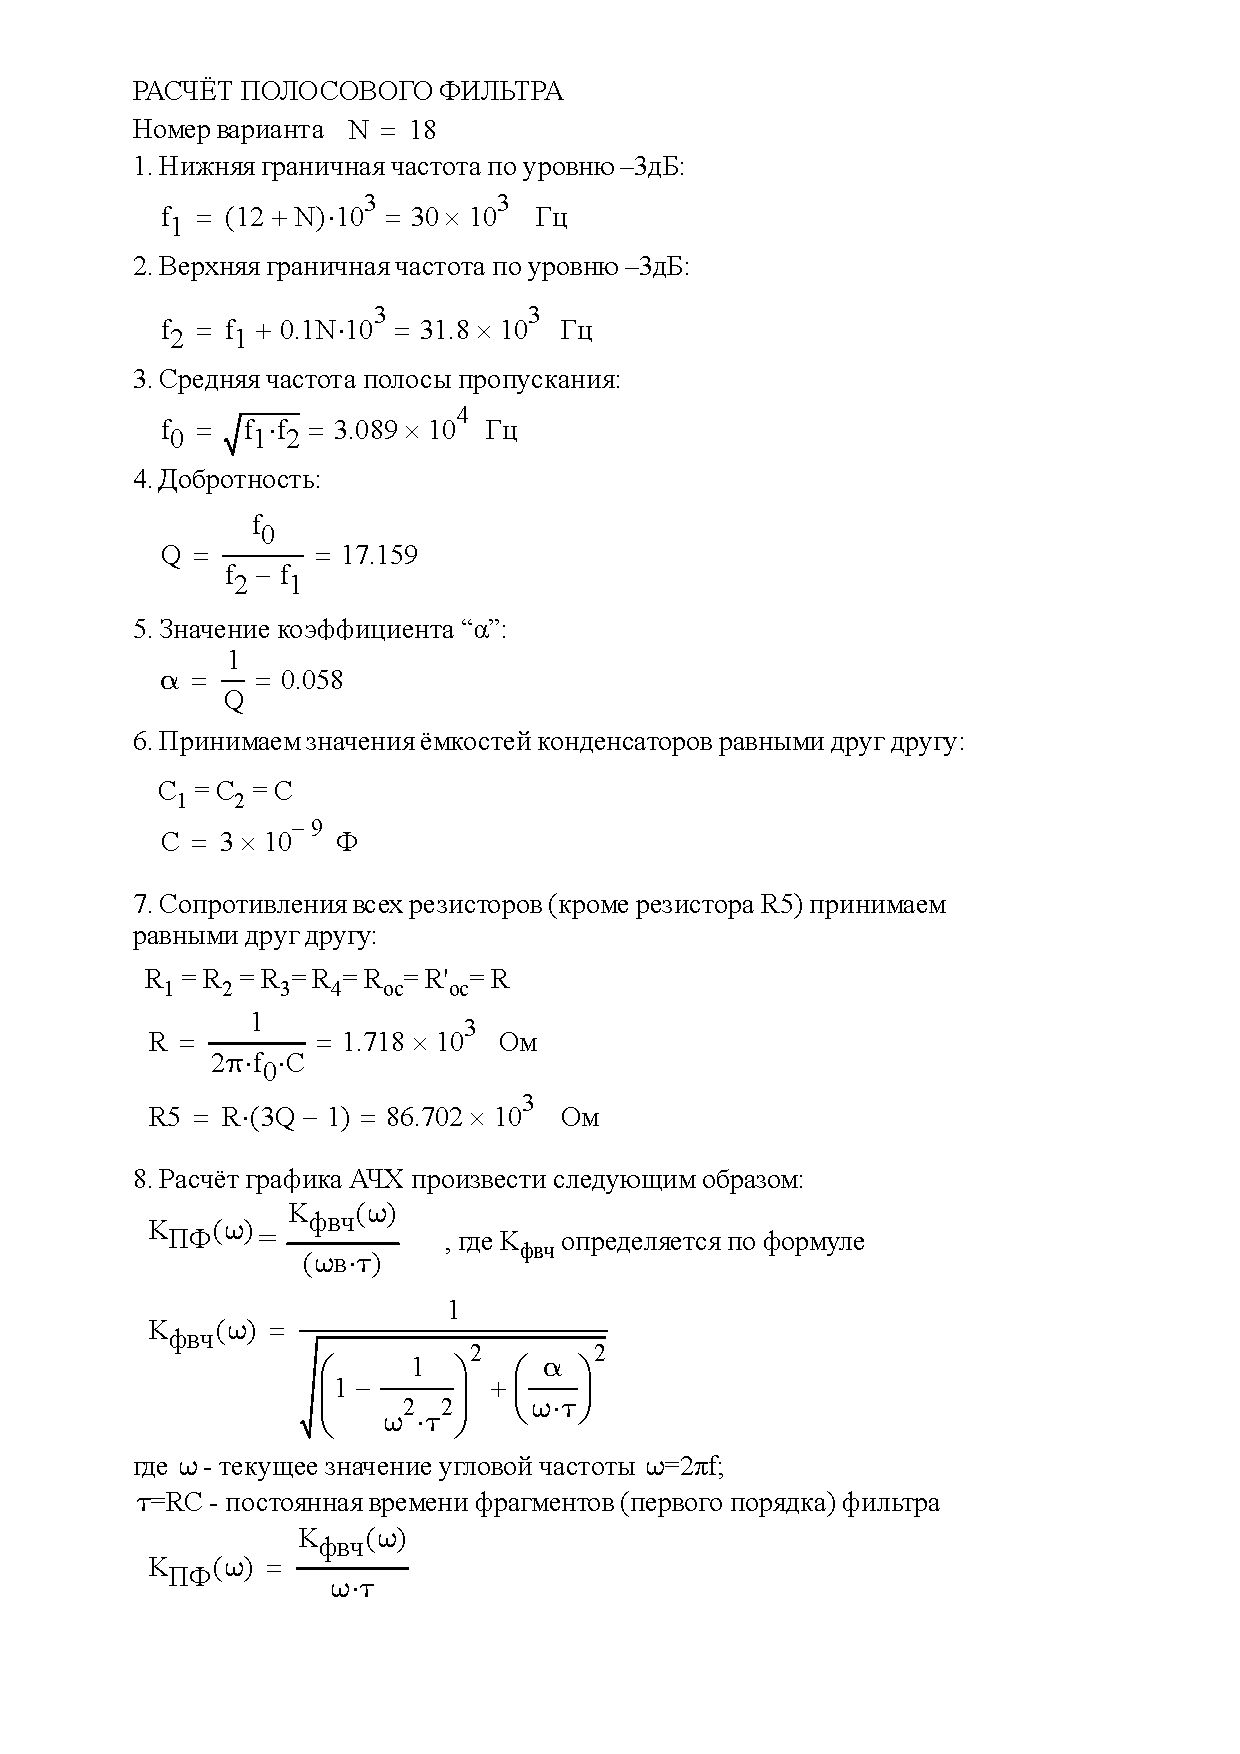
\includepdf[pages={1,3,5}]{myfile.pdf}
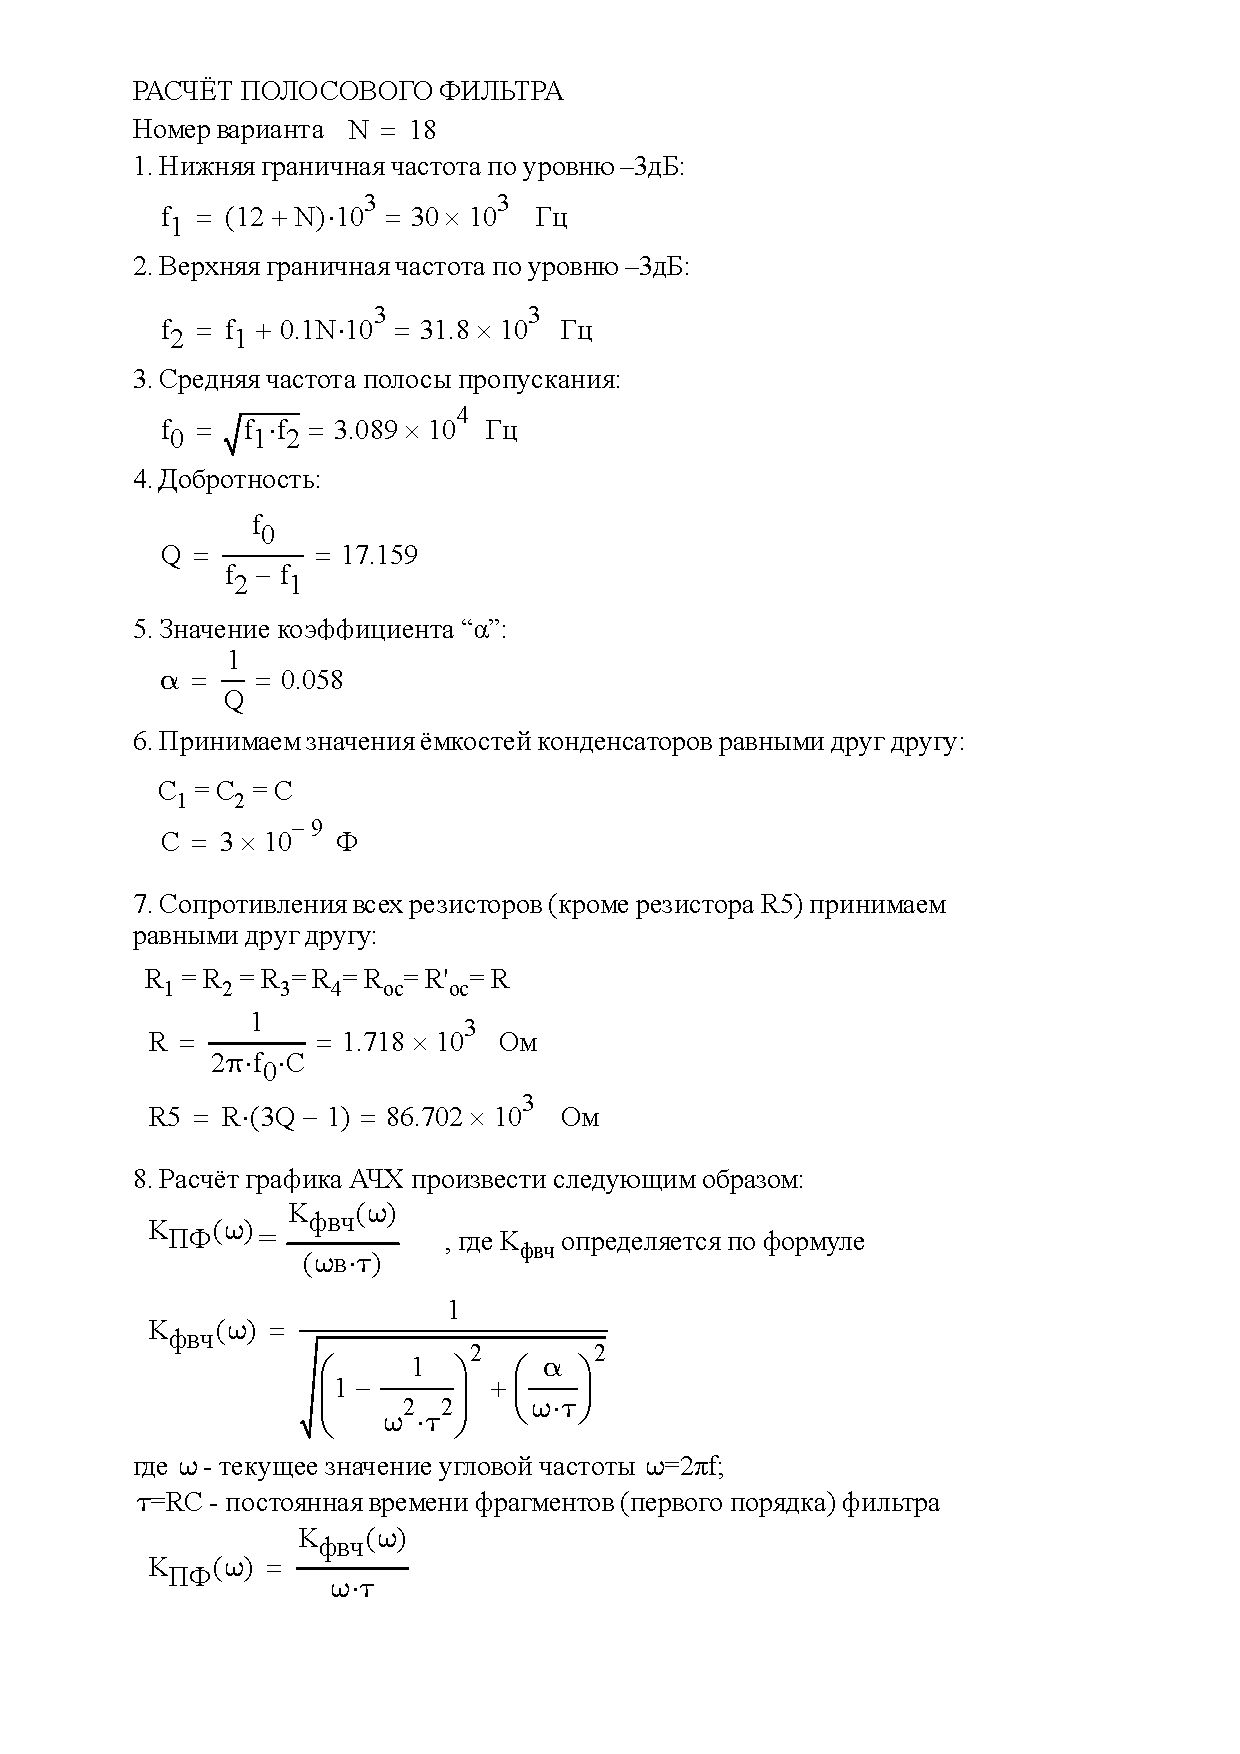
\includepdf[pages={-}]{myfile.pdf}



% \newpage
% \bibliographystyle{plain}
% \bibliography{bibliography}


\end{sloppypar}
